In all simulations, $L=1$, control input $u$ is limited in $U = [-\overline{u}, +\overline{u}]$ where $\overline{u}=1.5$ and the disturbance $d$ in $D=[-\overline{d}, +\overline{d}]$ where $\overline{d}=0.15$. In order to take into account robot dimensions in the configuration space ($\mathcal{C}$-space), we approximate its shape as a circle with $radius = (4/3)L$.

Our Simulations are divided in two main cases: 
\begin{itemize}
    \item The first one takes place in a static environment, where we have fixed obstacles and a fixed target set 
    \item The second one takes place in a dynamic environment with moving obstacles and a moving target set.
\end{itemize}
The second case contains three sub-cases:  
\begin{itemize}
    \item The Robot starts near the target set
    \item The Robot starts distant from the target set
    \item The Robot starts outside the $RAS$ (Reach-Avoid Set)
\end{itemize}
In addiction, for some simulations we test two disturbances strategies: 
\begin{itemize}
    \item Optimal Disturbance (\ref{opt_d})
    \item Random Disturbance 
\end{itemize}
The random disturbance is sampled from a Normal Gaussian distribution, with mean $\mu=0$ and standard deviation $\sigma=\overline{d}/3$. $\sigma$ has this form since in this way most of the samples ($99.7\%$) are in $D$, those outside are clipped.

All simulations have been implemented in Matlab using both ToolboxLS \cite{LS} and helperOC \cite{brief_intro} libraries. The code (\textit{main.m}) is available in the code folder.

\subsection{Static Case}
As mentioned before in this case the robot has to reach a fixed target set which is among some rectangular fixed obstacles. The simulation develops in a time of 10 seconds.
The first step is the computation of the value function $V^+(x,t)$ from which we can obtain the $RAS$, Figs. (\ref{fig:staticRAS3}), (\ref{fig:staticRAS2}), (\ref{fig:staticRAS1}) show the static environment in $\mathcal{C}$-space and $RAS$ regression during the game in different instants of time. The blue contour represents the border of $RAS$, so from any initial configuration $x_0 = [x_{r0},y_{r0},\theta_{r0}]^T$ inside the blue border our robot is expected to reach the target set in the time limit of 10 seconds despite the disturbance.   
\begin{figure}[h!]
    \centering
    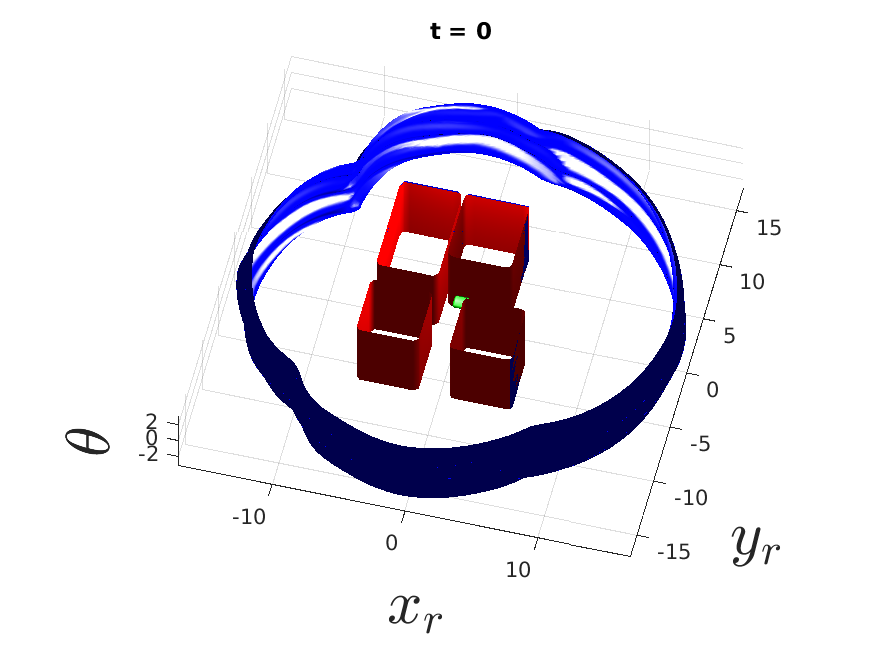
\includegraphics
        [width=0.4\textwidth]
        {figures/staticRAS3.png}
    \caption{Static environment and RAS at game start. The two horizontal axes represent the two first robot state components ($x_r$, $y_r$), while the third axis represents the third component $\theta$, namely the angle that the X-axis of $RF_m$ forms with $RF_w$. The small green cuboid represents the target set and the four red cuboids represents the obstacles. Since this representation takes place in $\mathcal{C}$-space the obstacles are bigger than their real dimensions in the workspace and the target set seems smaller. Blue contour indicates the border of RAS}
    \label{fig:staticRAS3}
\end{figure}
\begin{figure}[h!]
    \centering
    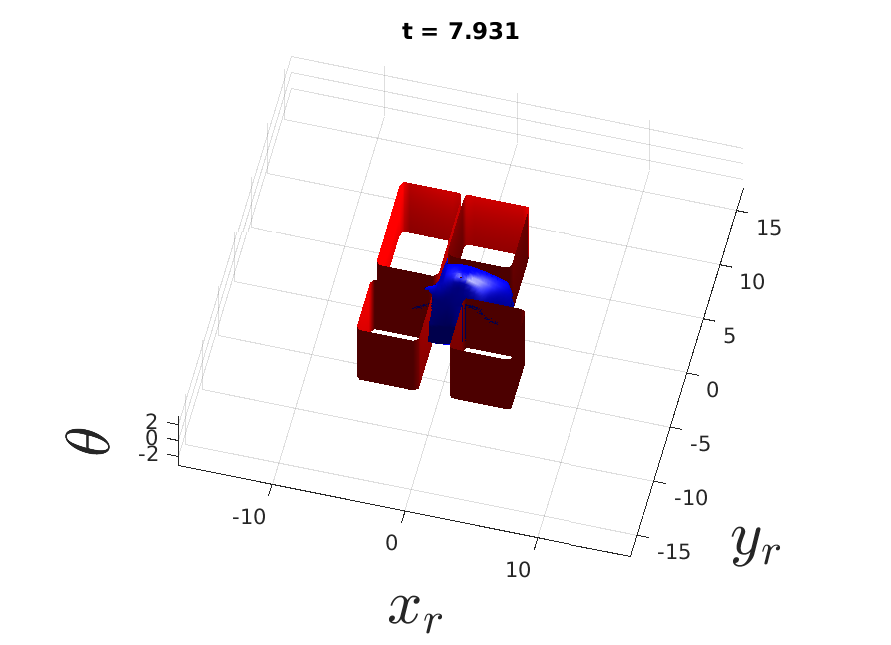
\includegraphics
        [width=0.4\textwidth]
        {figures/staticRAS2.png}
    \caption{Static environment and RAS at time 7.931s}
    \label{fig:staticRAS2}
\end{figure}
\begin{figure}[h!]
    \centering
    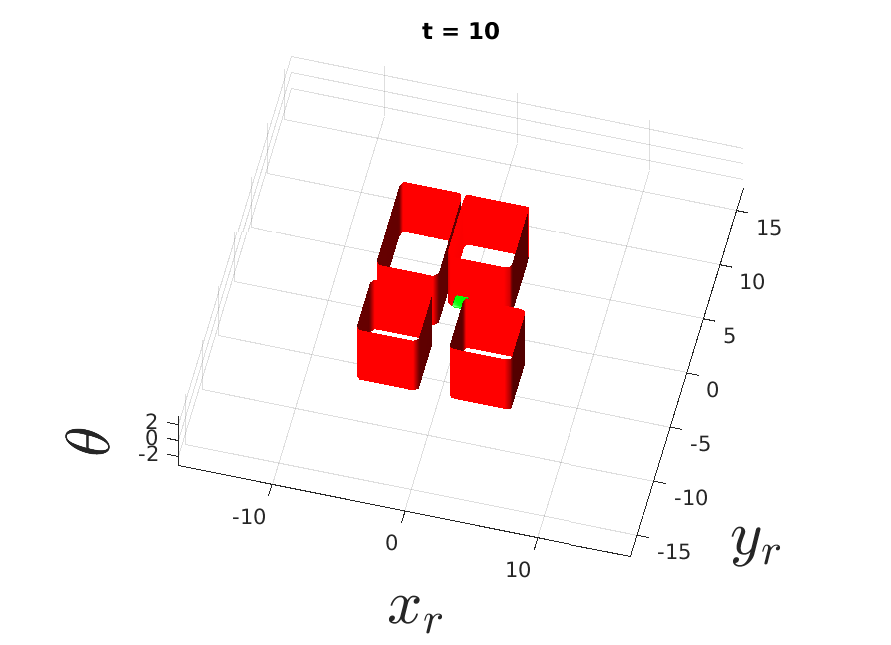
\includegraphics
        [width=0.4\textwidth]
        {figures/staticRAS1.png}
    \caption{Static environment and RAS (empty) at end game}
    \label{fig:staticRAS1}
\end{figure}

In $\mathcal{C}$-space the target set has a limited height $\theta \in [-0.1, 0.1]$ since we want the robot reaches the target set with a desired orientation $\theta_d$ in a small range around $0\,rad$.

Now that the $RAS$ is defined we can see how the robot, starting from an initial state $x_0$ at time $t=0$, reaches the target set avoiding obstacles despite the disturbance. So since the robot's initial position $x_0 = [-5, -8 -2]$ is in the limits of the $RAS$ we can see that it reaches, after the needed time, the target set in the desired orientation, avoiding the obstacles in its path. Fig. (\ref{fig:static_opt}) shows the trajectory in both configuration and work-space and also the optimal player moves at each time instant of the game. In Fig. (\ref{fig:static_random}) is shown the same experiment but instead of an optimal disturbance we use a random one.


%\pagebreak
%\clearpage
%\newpage
\subsection{Dynamic Case}
Now we will see some more complex cases where reach set and avoid set are not fixed, but they move in the environment. Here we simulated a moving platform which represent a recharging station for the robot. So the robot has to access the platform while this platform is moving downward along the Y-axis with a constant velocity $v=-1$. The platform is not accessible from everywhere, but only from the right side, while the other sides are surrounded by barriers (obstacles). The final desired orientation is the same of static environment ($\theta_d \in [-0.1, 0.1]$), so the target set is not restricted only in small area of the X-axis and Y-axis, but also in terms of the third component $\theta$.

As done before, the first step is the computation of RAS at each instant of the game, in this case we are going to see the $RAS$ regressing over time in a particular direction since the target set, always represented by a green area, can be reached from only one side, see Figs. (\ref{fig:ras_dyn_1.png}), (\ref{fig:ras_dyn_2.png}), (\ref{fig:ras_dyn_3.png}).

\begin{figure}[h!]
    \centering
    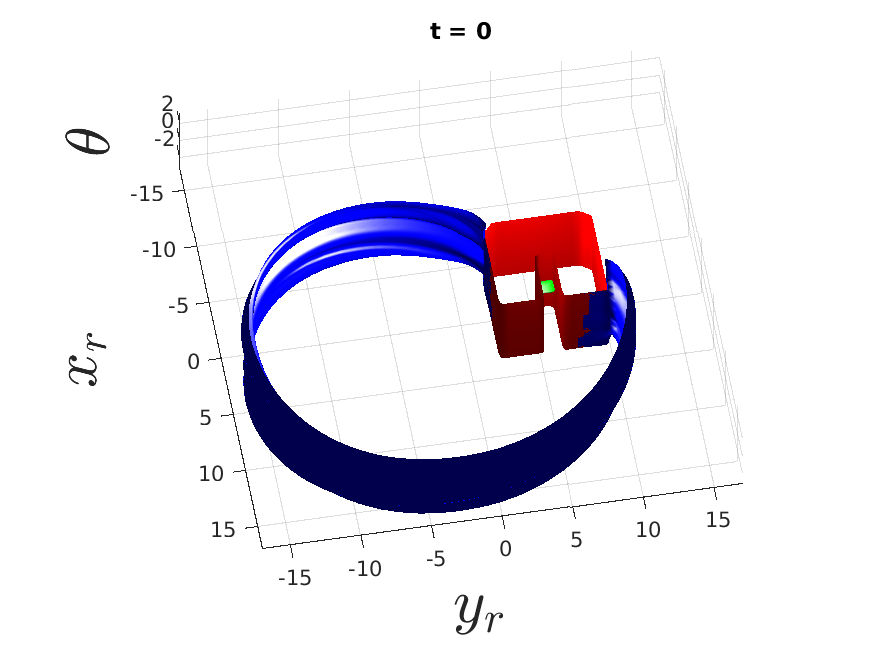
\includegraphics
        [width=0.4\textwidth]
        {figures/ras_dyn_1.png}
    \caption{Dynamic environment and RAS at game start}
    \label{fig:ras_dyn_1.png}
\end{figure}
\begin{figure}[h!]
    \centering
    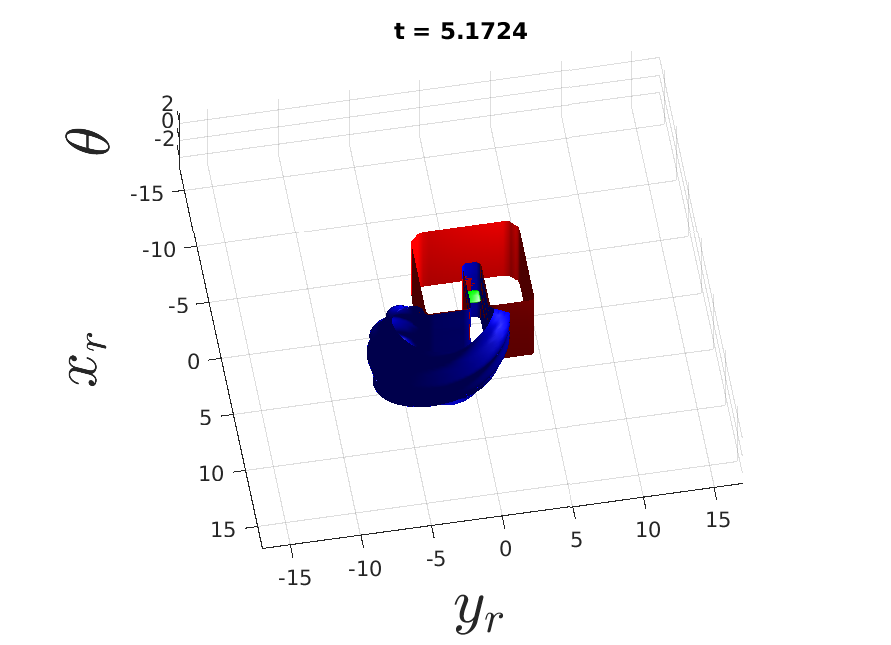
\includegraphics
        [width=0.4\textwidth]
        {figures/ras_dyn_2.png}
    \caption{Dynamic environment and RAS at time 5.1724s}
    \label{fig:ras_dyn_2.png}
\end{figure}
\begin{figure}[h!]
    \centering
    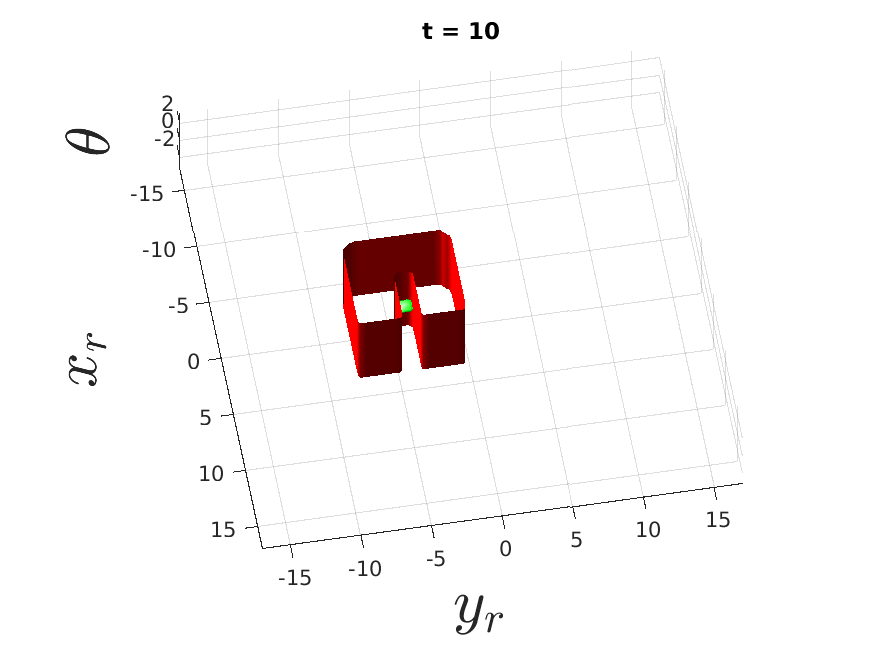
\includegraphics
        [width=0.4\textwidth]
        {figures/ras_dyn_3.png}
    \caption{Dynamic environment and RAS (empty) at end game}
    \label{fig:ras_dyn_3.png}
\end{figure}

As mentioned before, we simulated three different cases for the Dynamic experiments. 

\subsubsection{Case 1}
In this first case the initial position of the robot $x_0 = [0, 0, -3]$ is relatively near the target set and inside the $RAS$ at time 0, so we know from the theory that exists a trajectory which can lead the robot inside the target set in the maximum given time (10 seconds).
In Fig. (\ref{fig:dynamic_closer_opt}) we can see the particular trajectory of the robot necessary to reach the moving target set despite an optimal disturbance. As expected, at time 10 the robot is in the target set with the desired orientation without collisions with the obstacles.

\subsubsection{Case 2}
The second case is similar to the previous one, the only difference is the initial position of the robot ($x_0 = [0, -7, -3]$). Here the robot is relatively distant from the target set, but still in the $RAS$. Even in this case the robot successfully reached the target set with the desired angle $\theta_d$, playing against the optimal disturbance and avoiding any obstacle (Fig. (\ref{fig:dynamic_faraway})). The robot trajectory when the disturbance acts random is shown in Fig. (\ref{fig:dynamic_faraway_ran}).  

\subsubsection{Case 3}
In this last case we see for completeness what happens if the initial position of the robot is outside the $RAS$. The initial position of the robot is $x_0 = [14, 14, -3]$, so completely outside the bounds of the RAS, obviously we can already say that the robot is not going to reach the target set.

As we can see from Fig. (\ref{fig:dynamic_outside_reach_avoid_set}), robot tries to reach the target but at time 10 it is still outside.
        

\begin{figure*}[hp!]
    \centering
    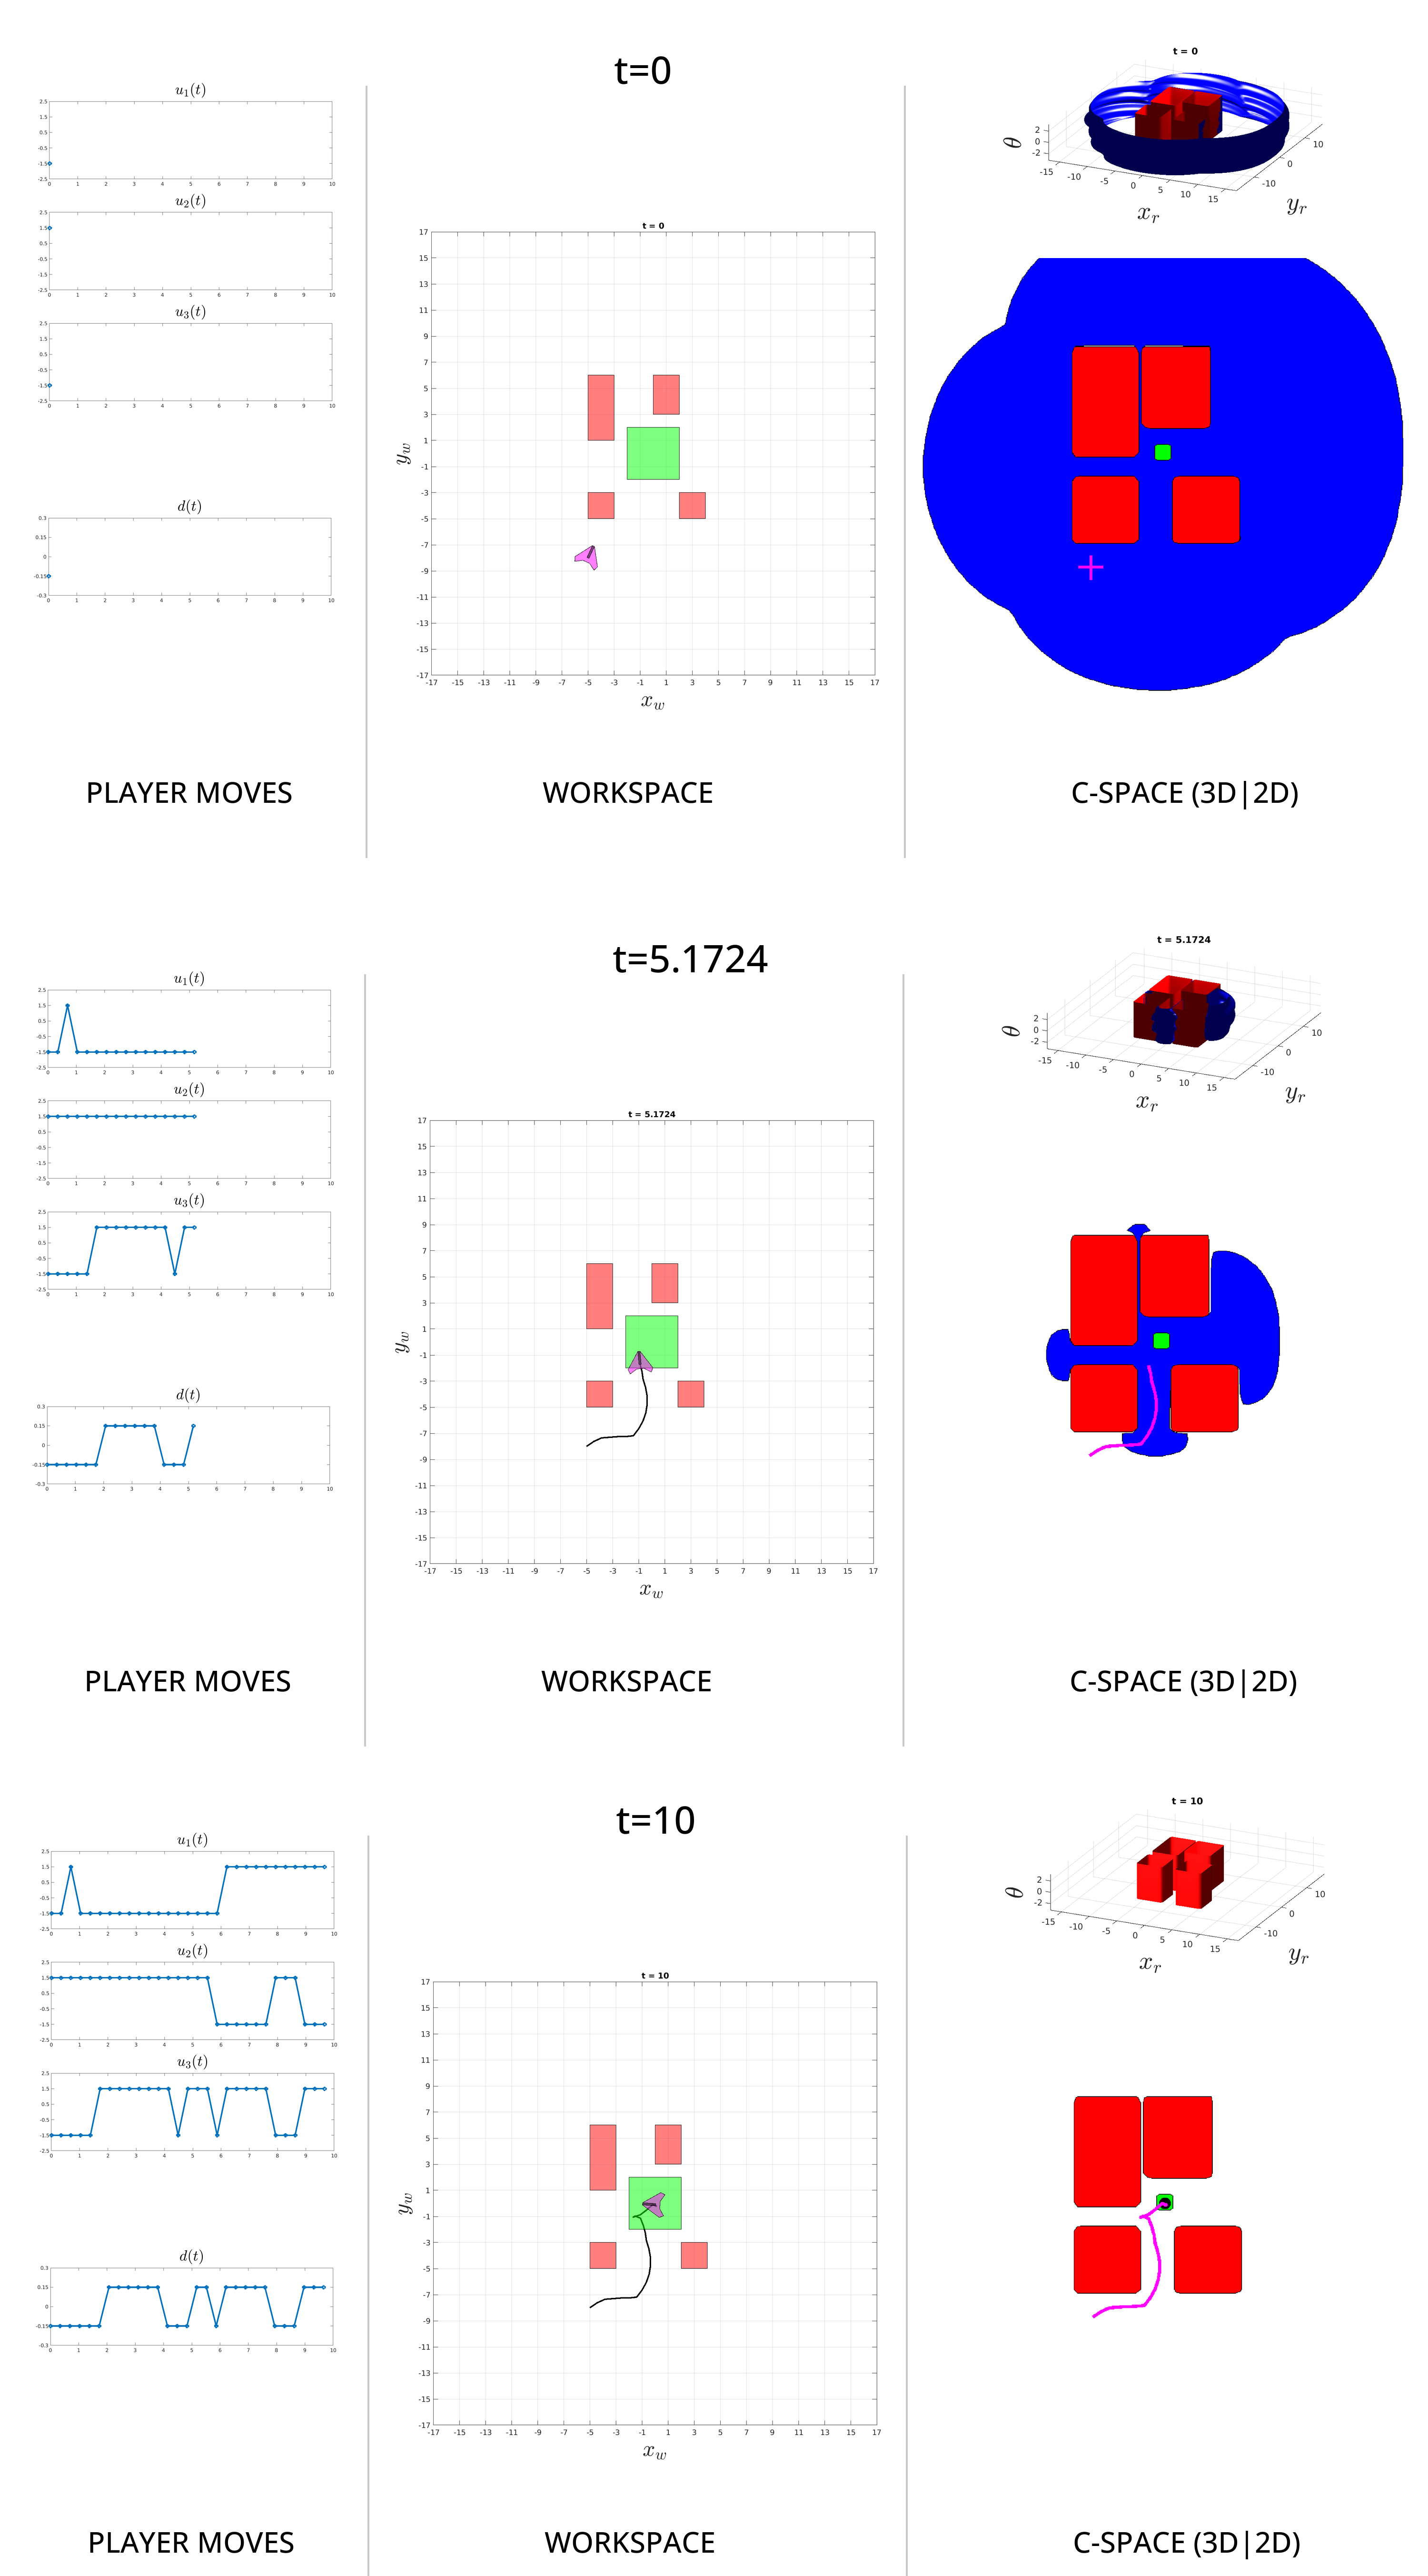
\includegraphics
        [width=0.7\textwidth]
        {figures/static_opt.png}
    \caption{Static environment, optimal disturbance. $x_0 = [-5, -8 -2]$, $\theta_d \in [-0.1, 0.1]$}
    \label{fig:static_opt}
\end{figure*}
\begin{figure*}[hp!]
    \centering
    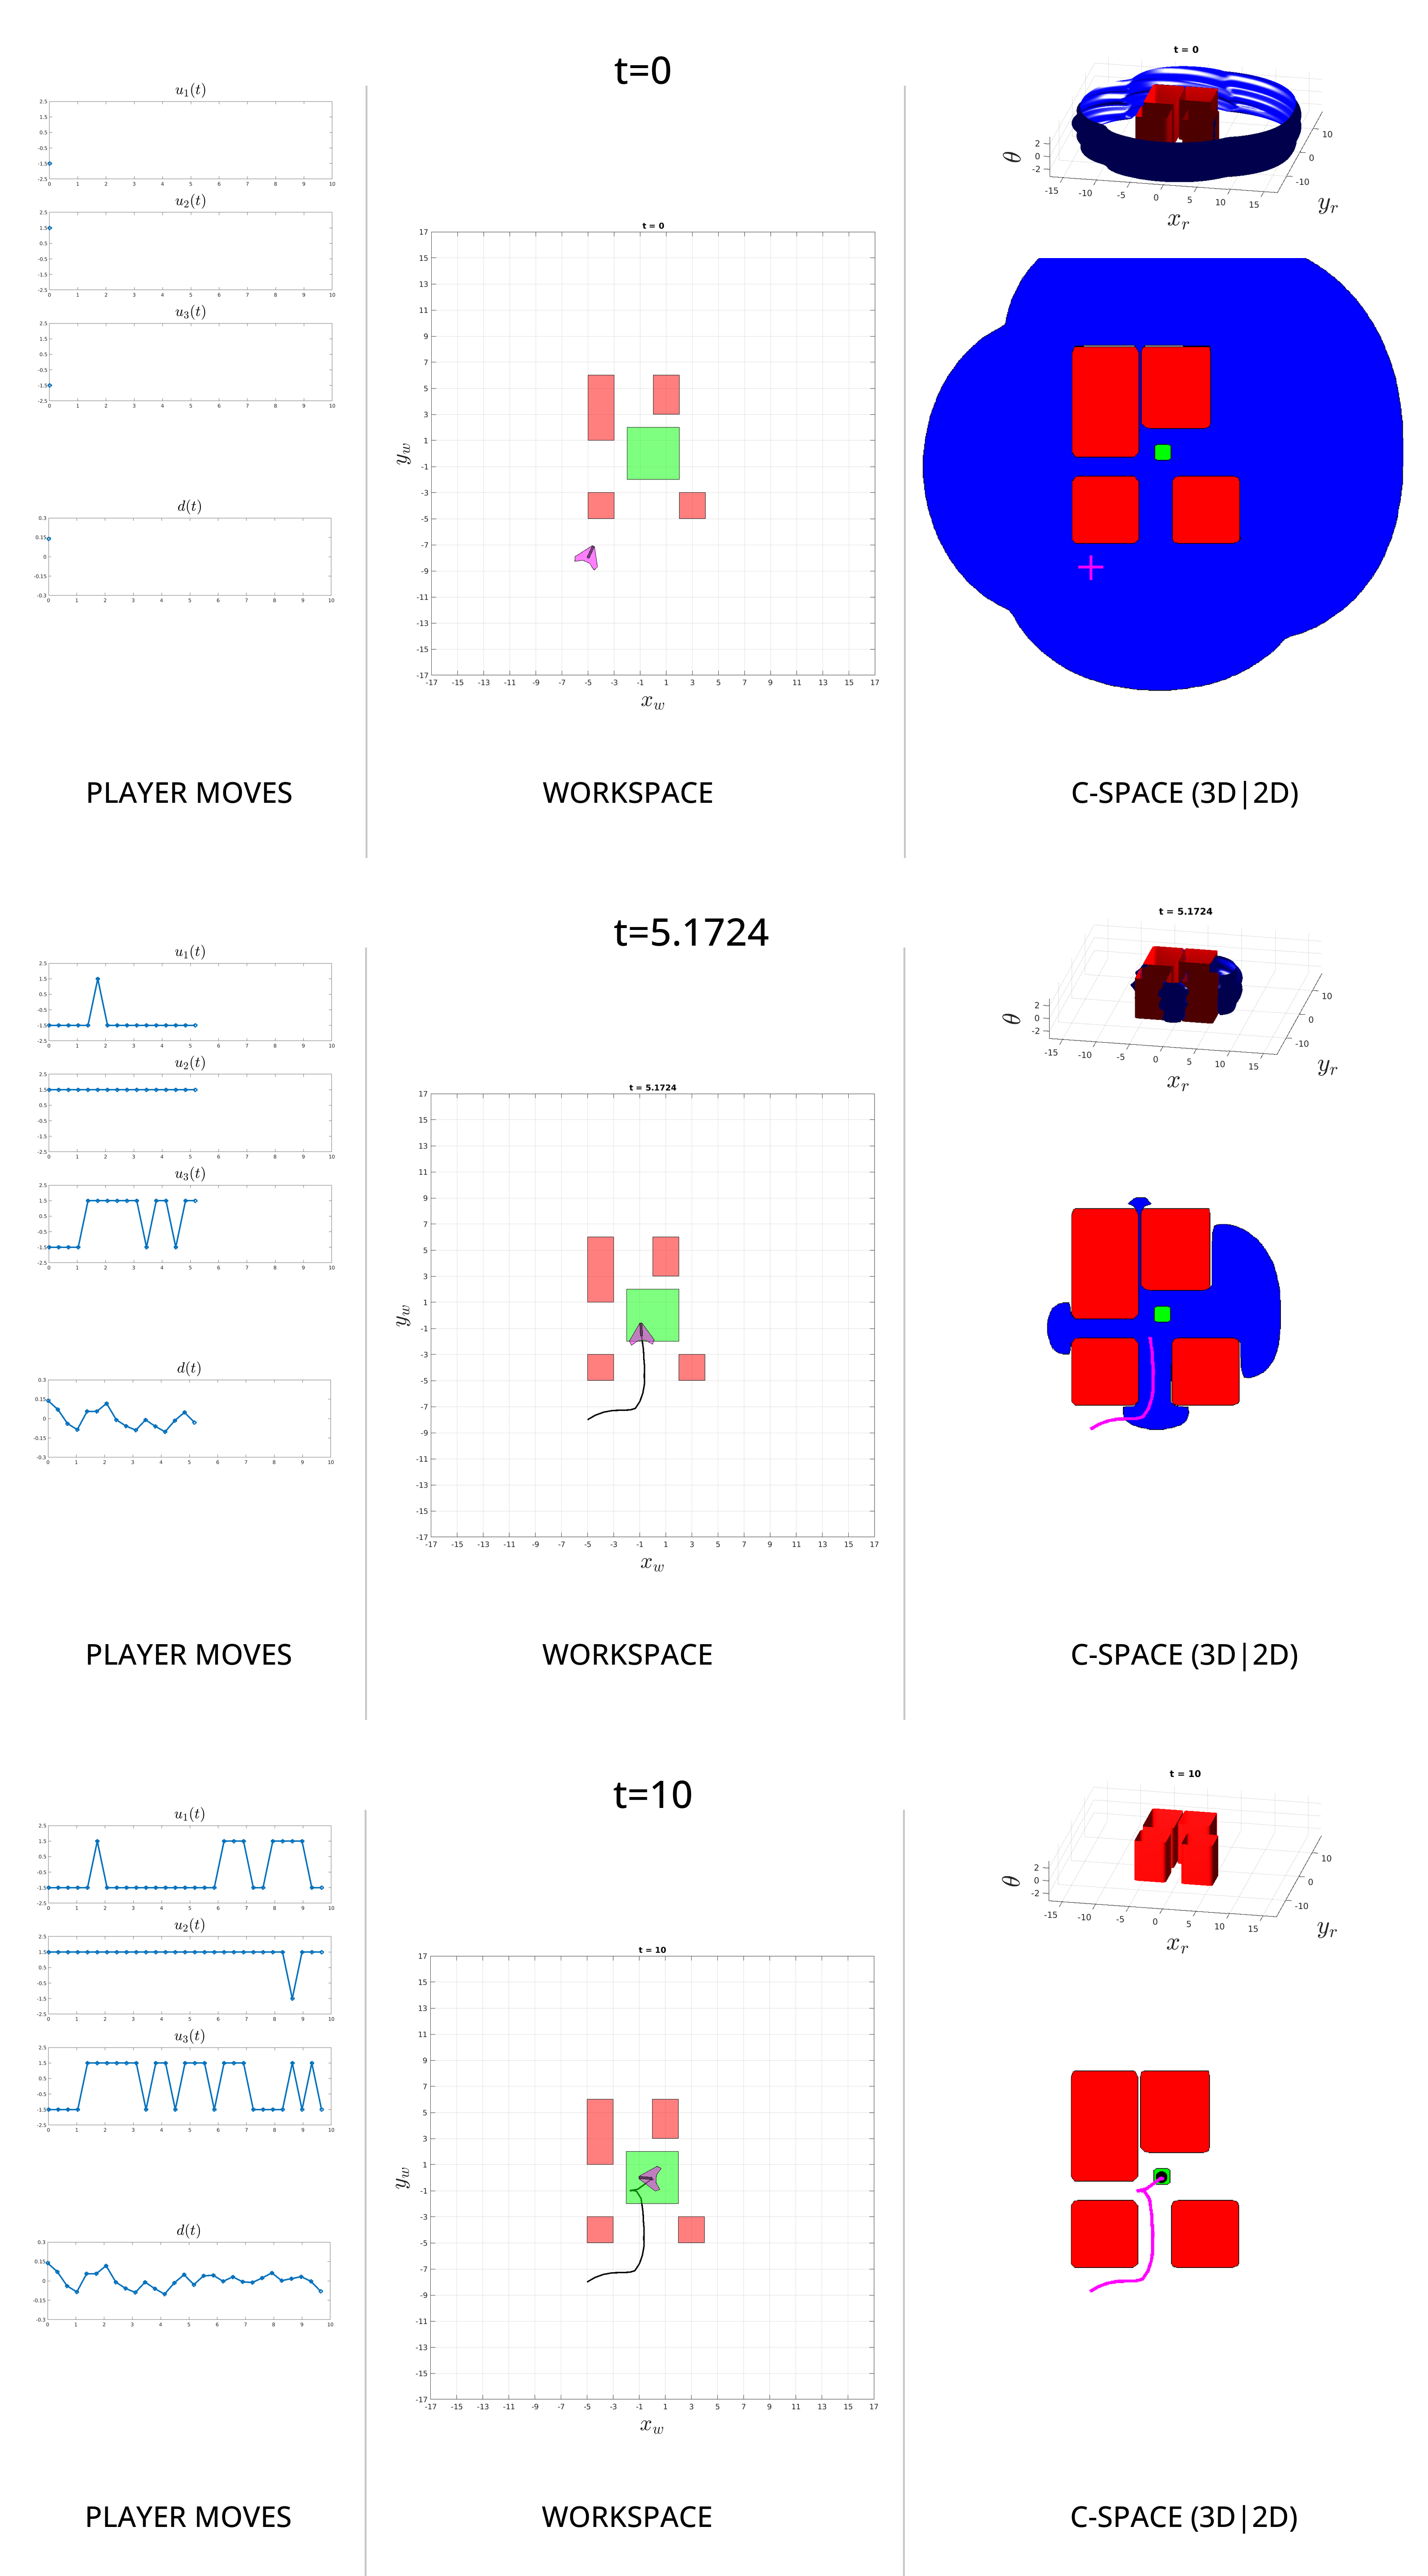
\includegraphics
        [width=0.7\textwidth]
        {figures/static_random.png}
    \caption{Static environment, random disturbance. $x_0 = [-5, -8 -2]$, $\theta_d \in [-0.1, 0.1]$}
    \label{fig:static_random}
\end{figure*}

\begin{figure*}[hp!]
    \centering
    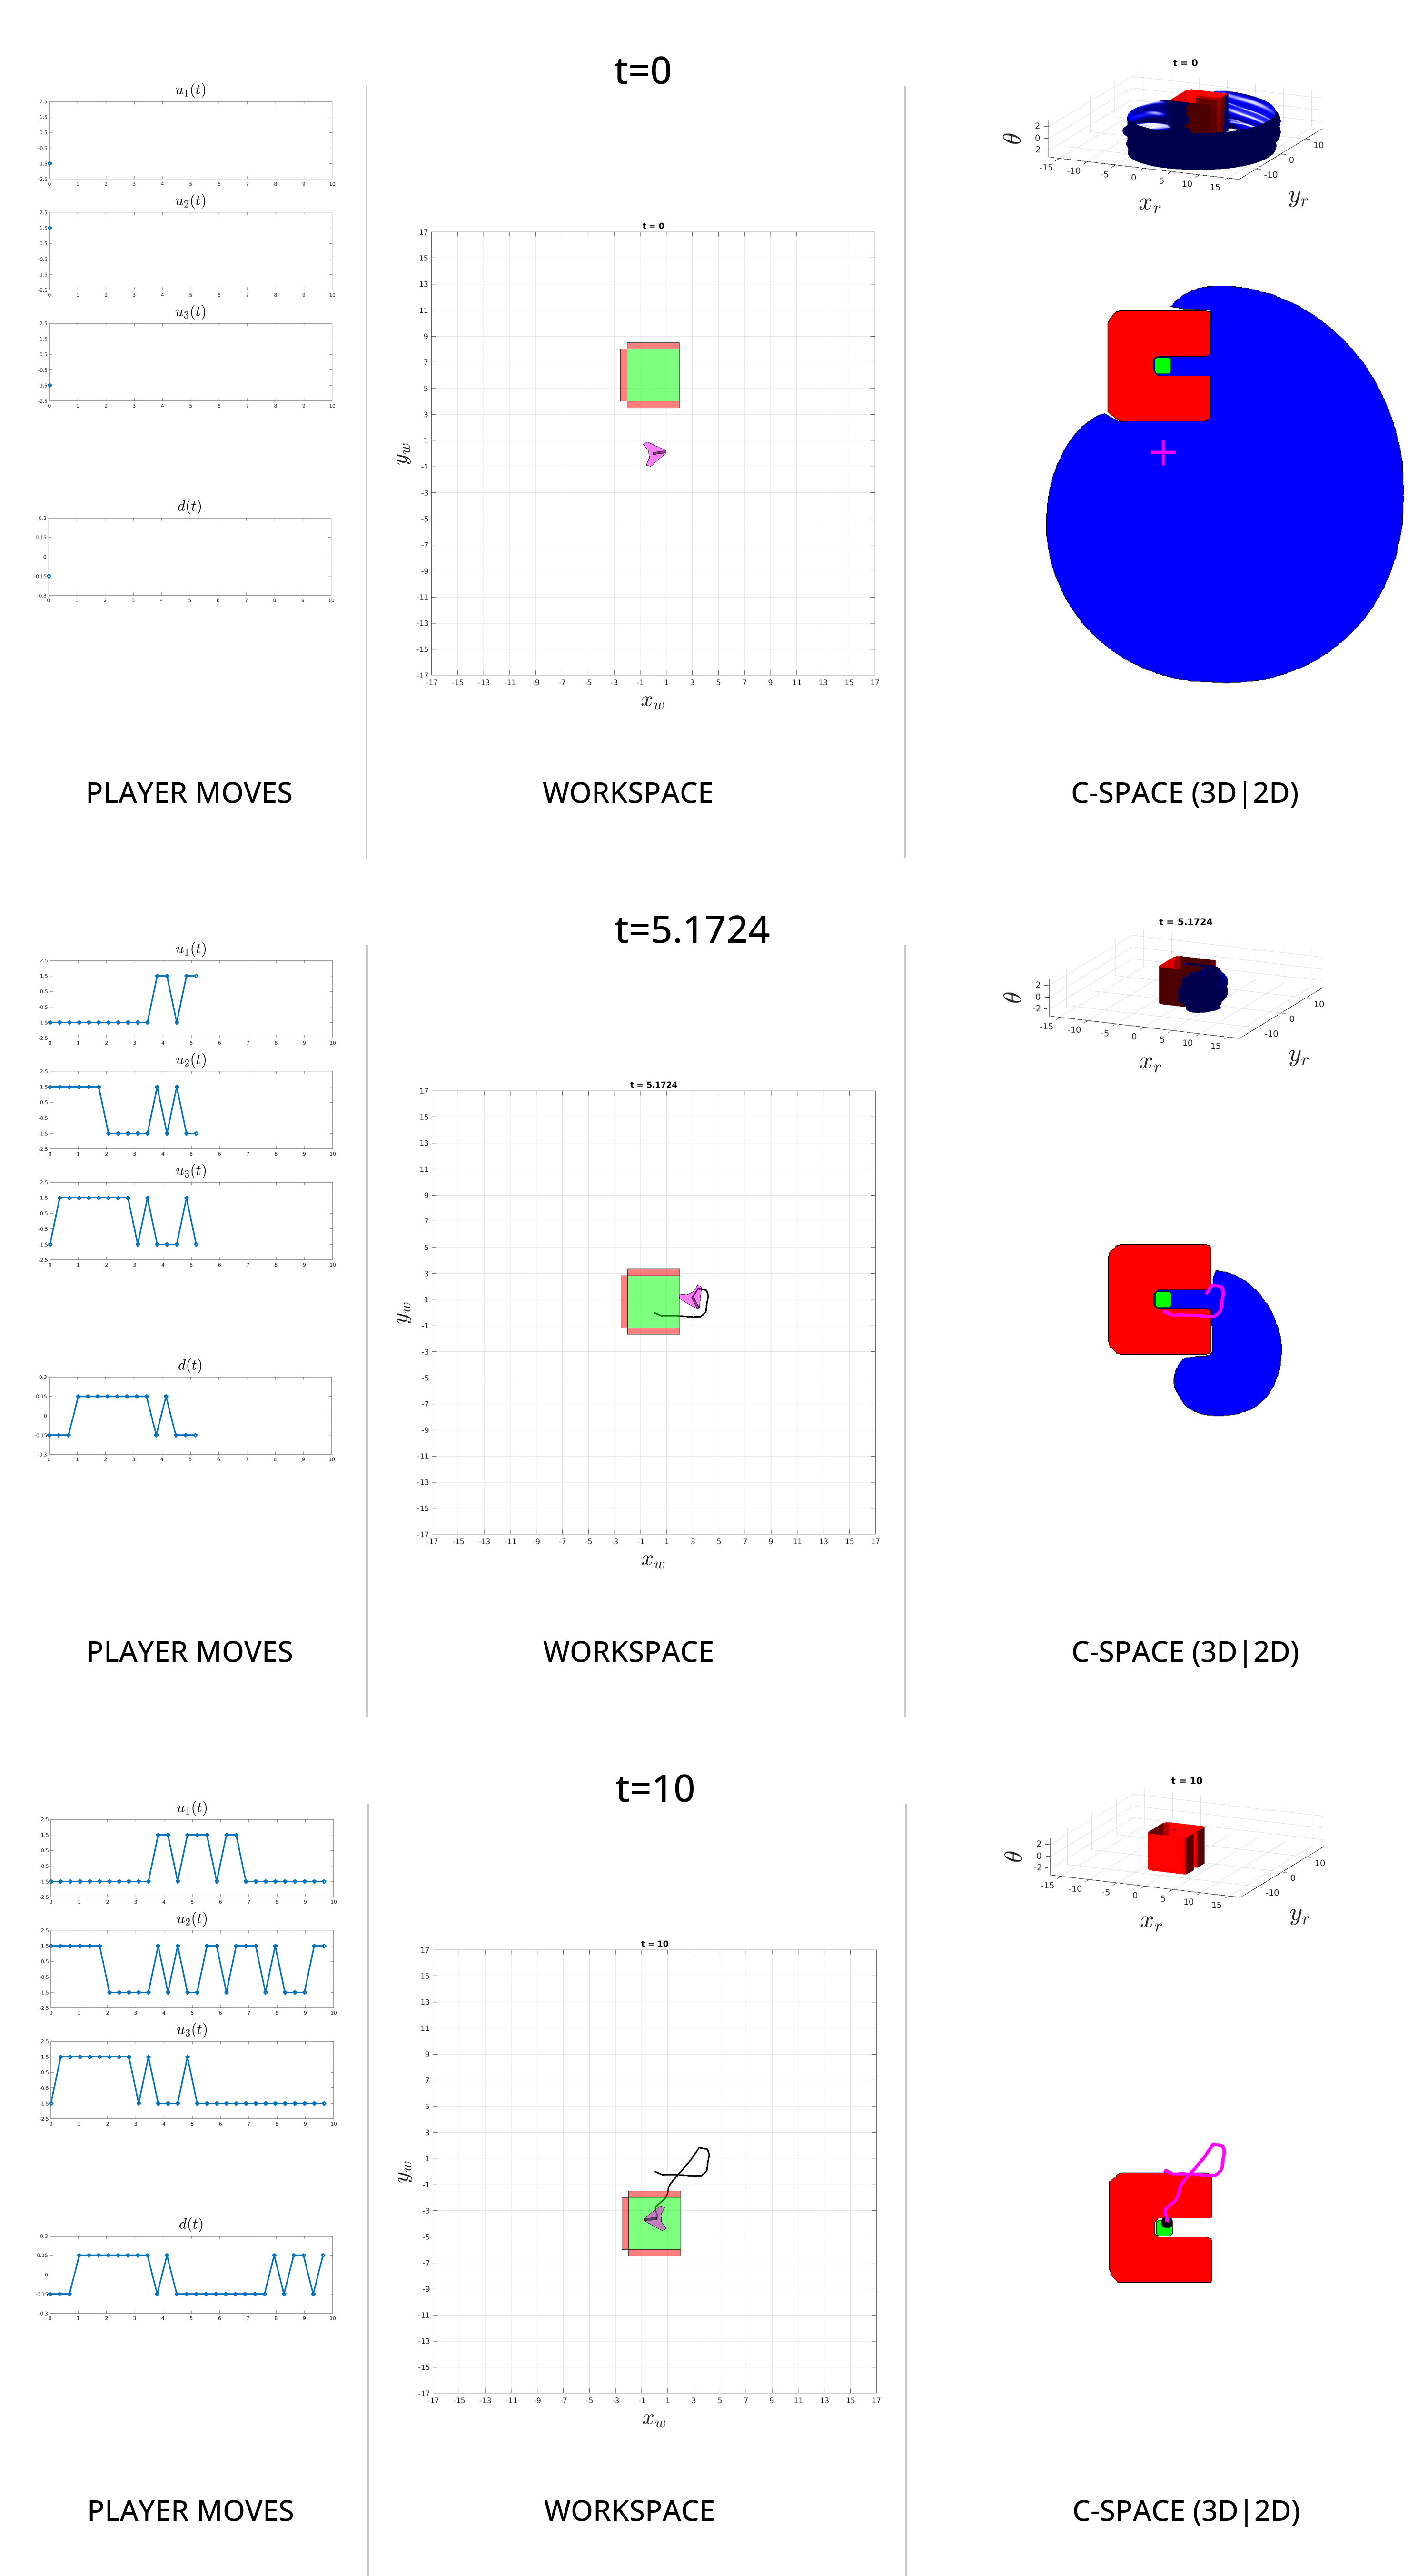
\includegraphics
        [width=0.7\textwidth]
        {figures/dynamic_closer_opt.png}
    \caption{Dynamic environment, optimal disturbance. $x_0 = [0, 0, -3]$, $\theta_d \in [-0.1, 0.1]$}
    \label{fig:dynamic_closer_opt}
\end{figure*}

\begin{figure*}[hp!]
    \centering
    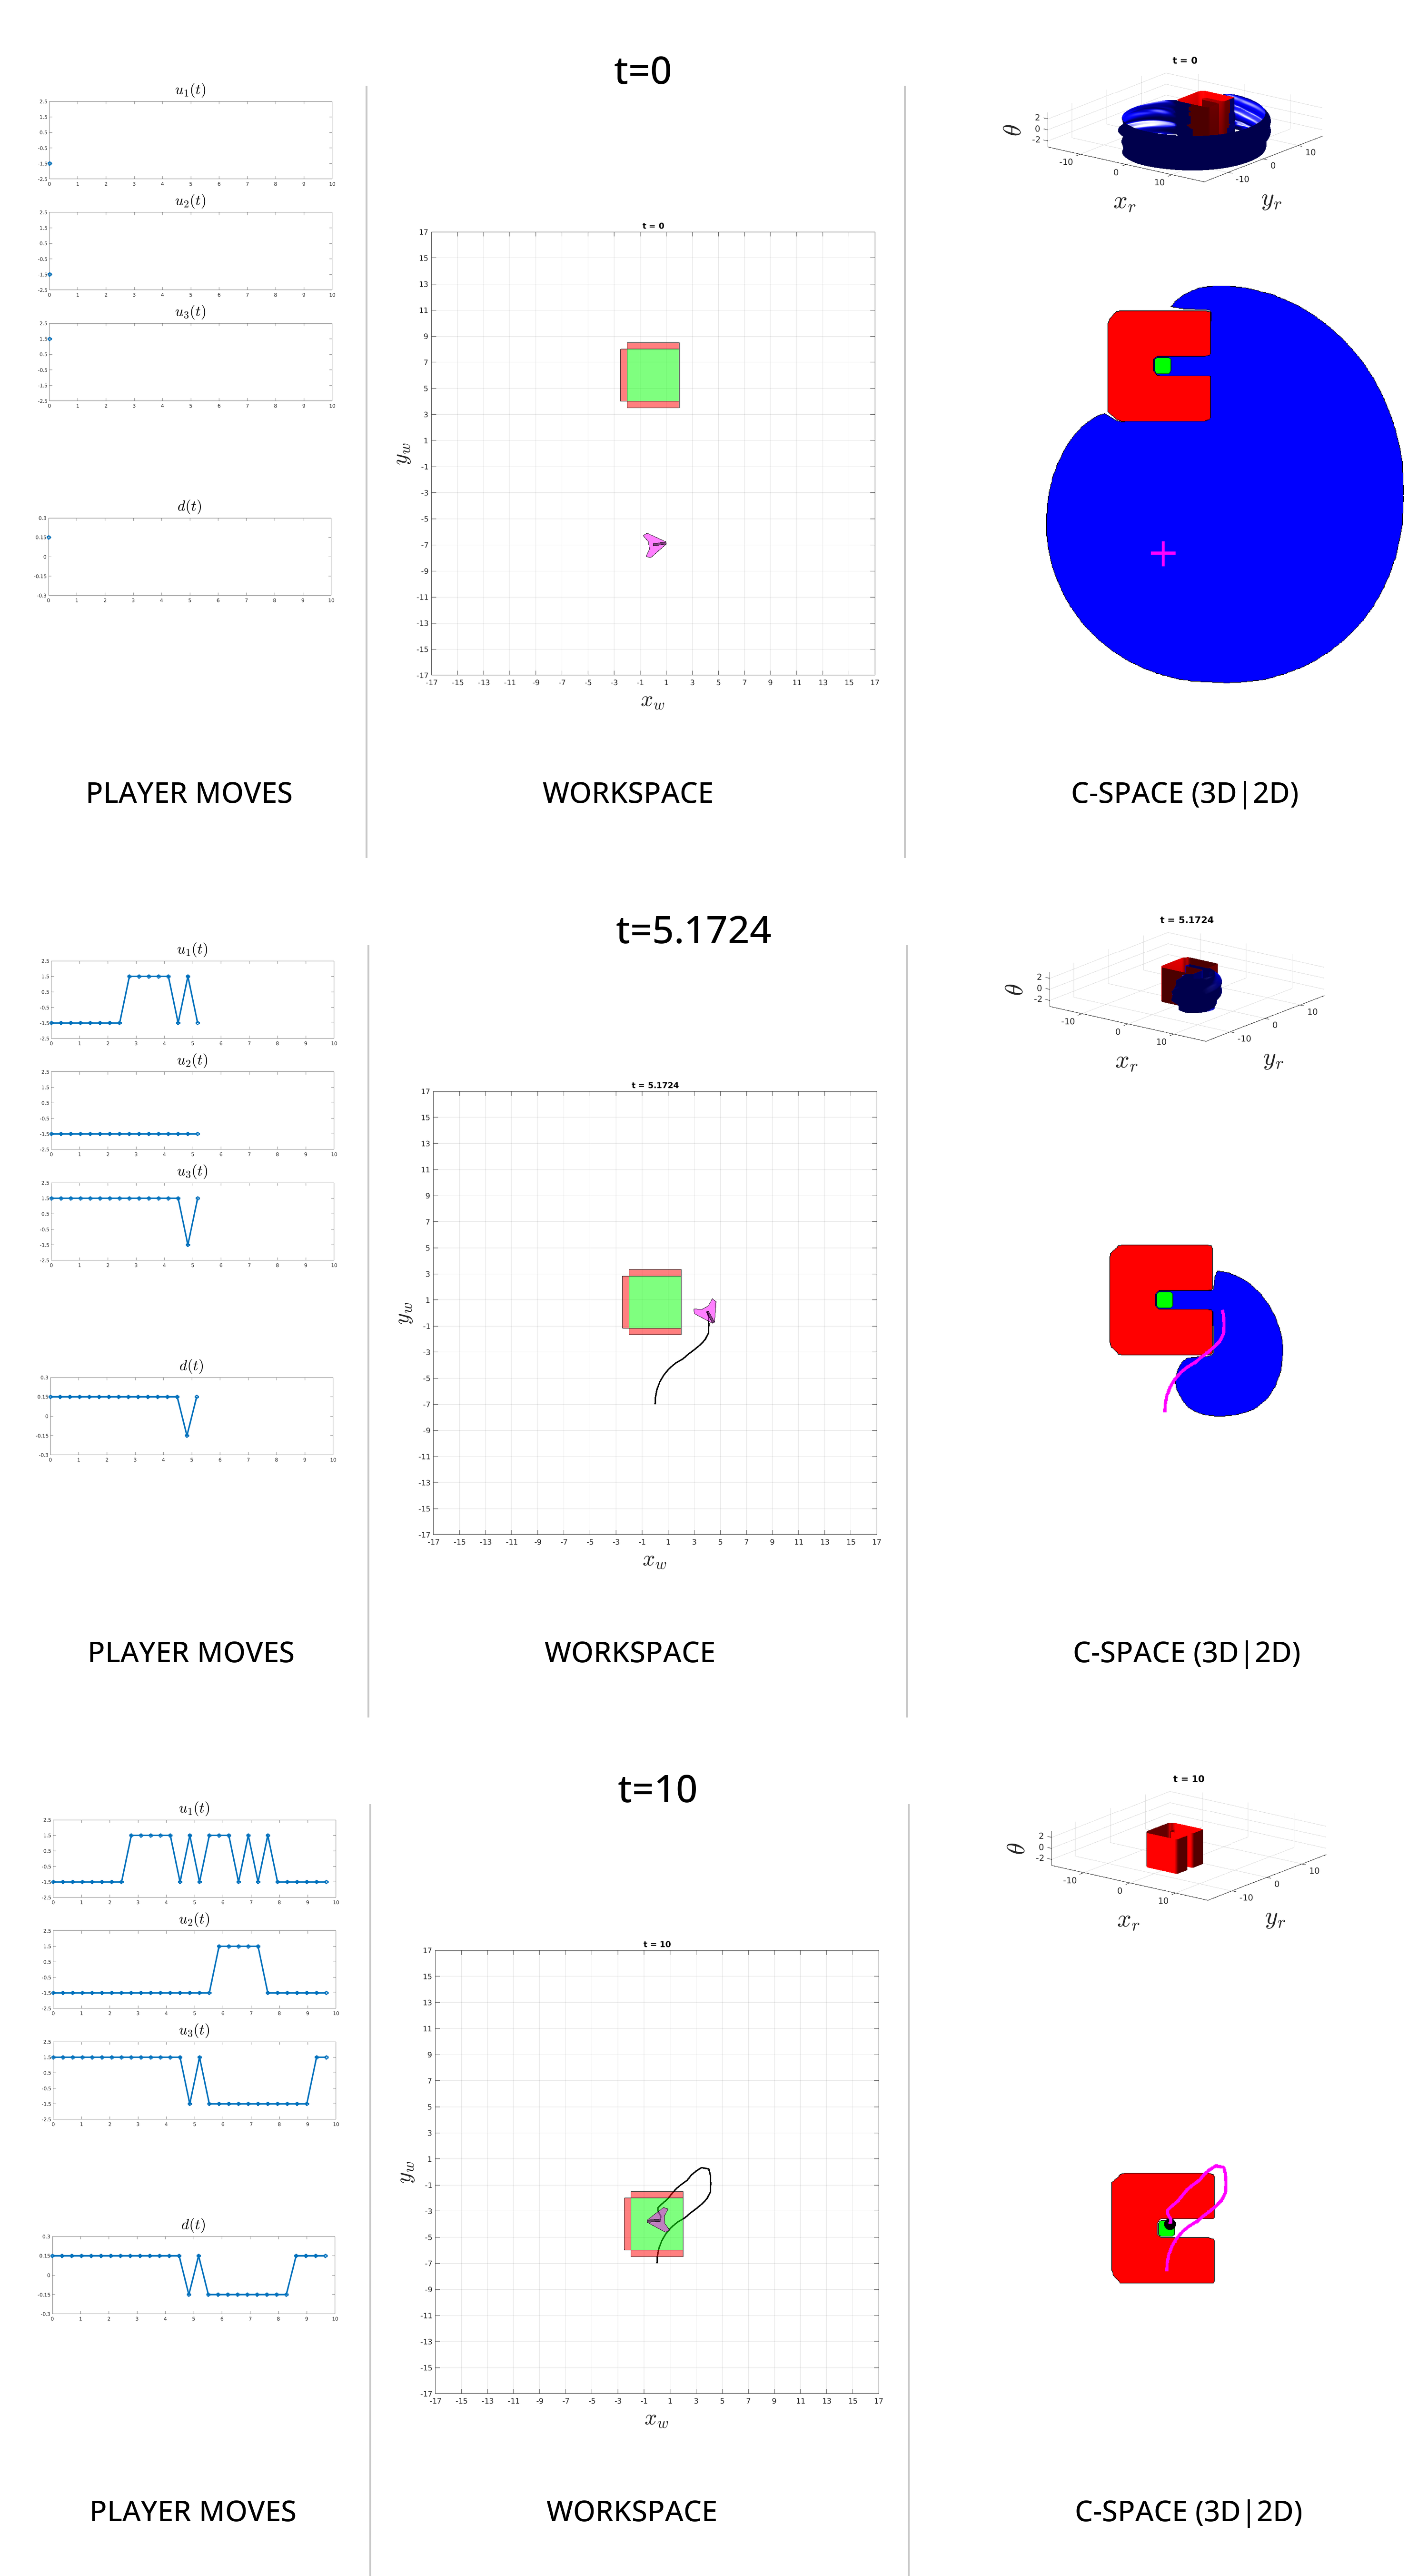
\includegraphics
        [width=0.7\textwidth]
        {figures/dynamic_faraway.png}
    \caption{Dynamic environment, optimal disturbance. $x_0 = [0, -7, -3]$, $\theta_d \in [-0.1, 0.1]$}
    \label{fig:dynamic_faraway}
\end{figure*}

\begin{figure*}[hp!]
    \centering
    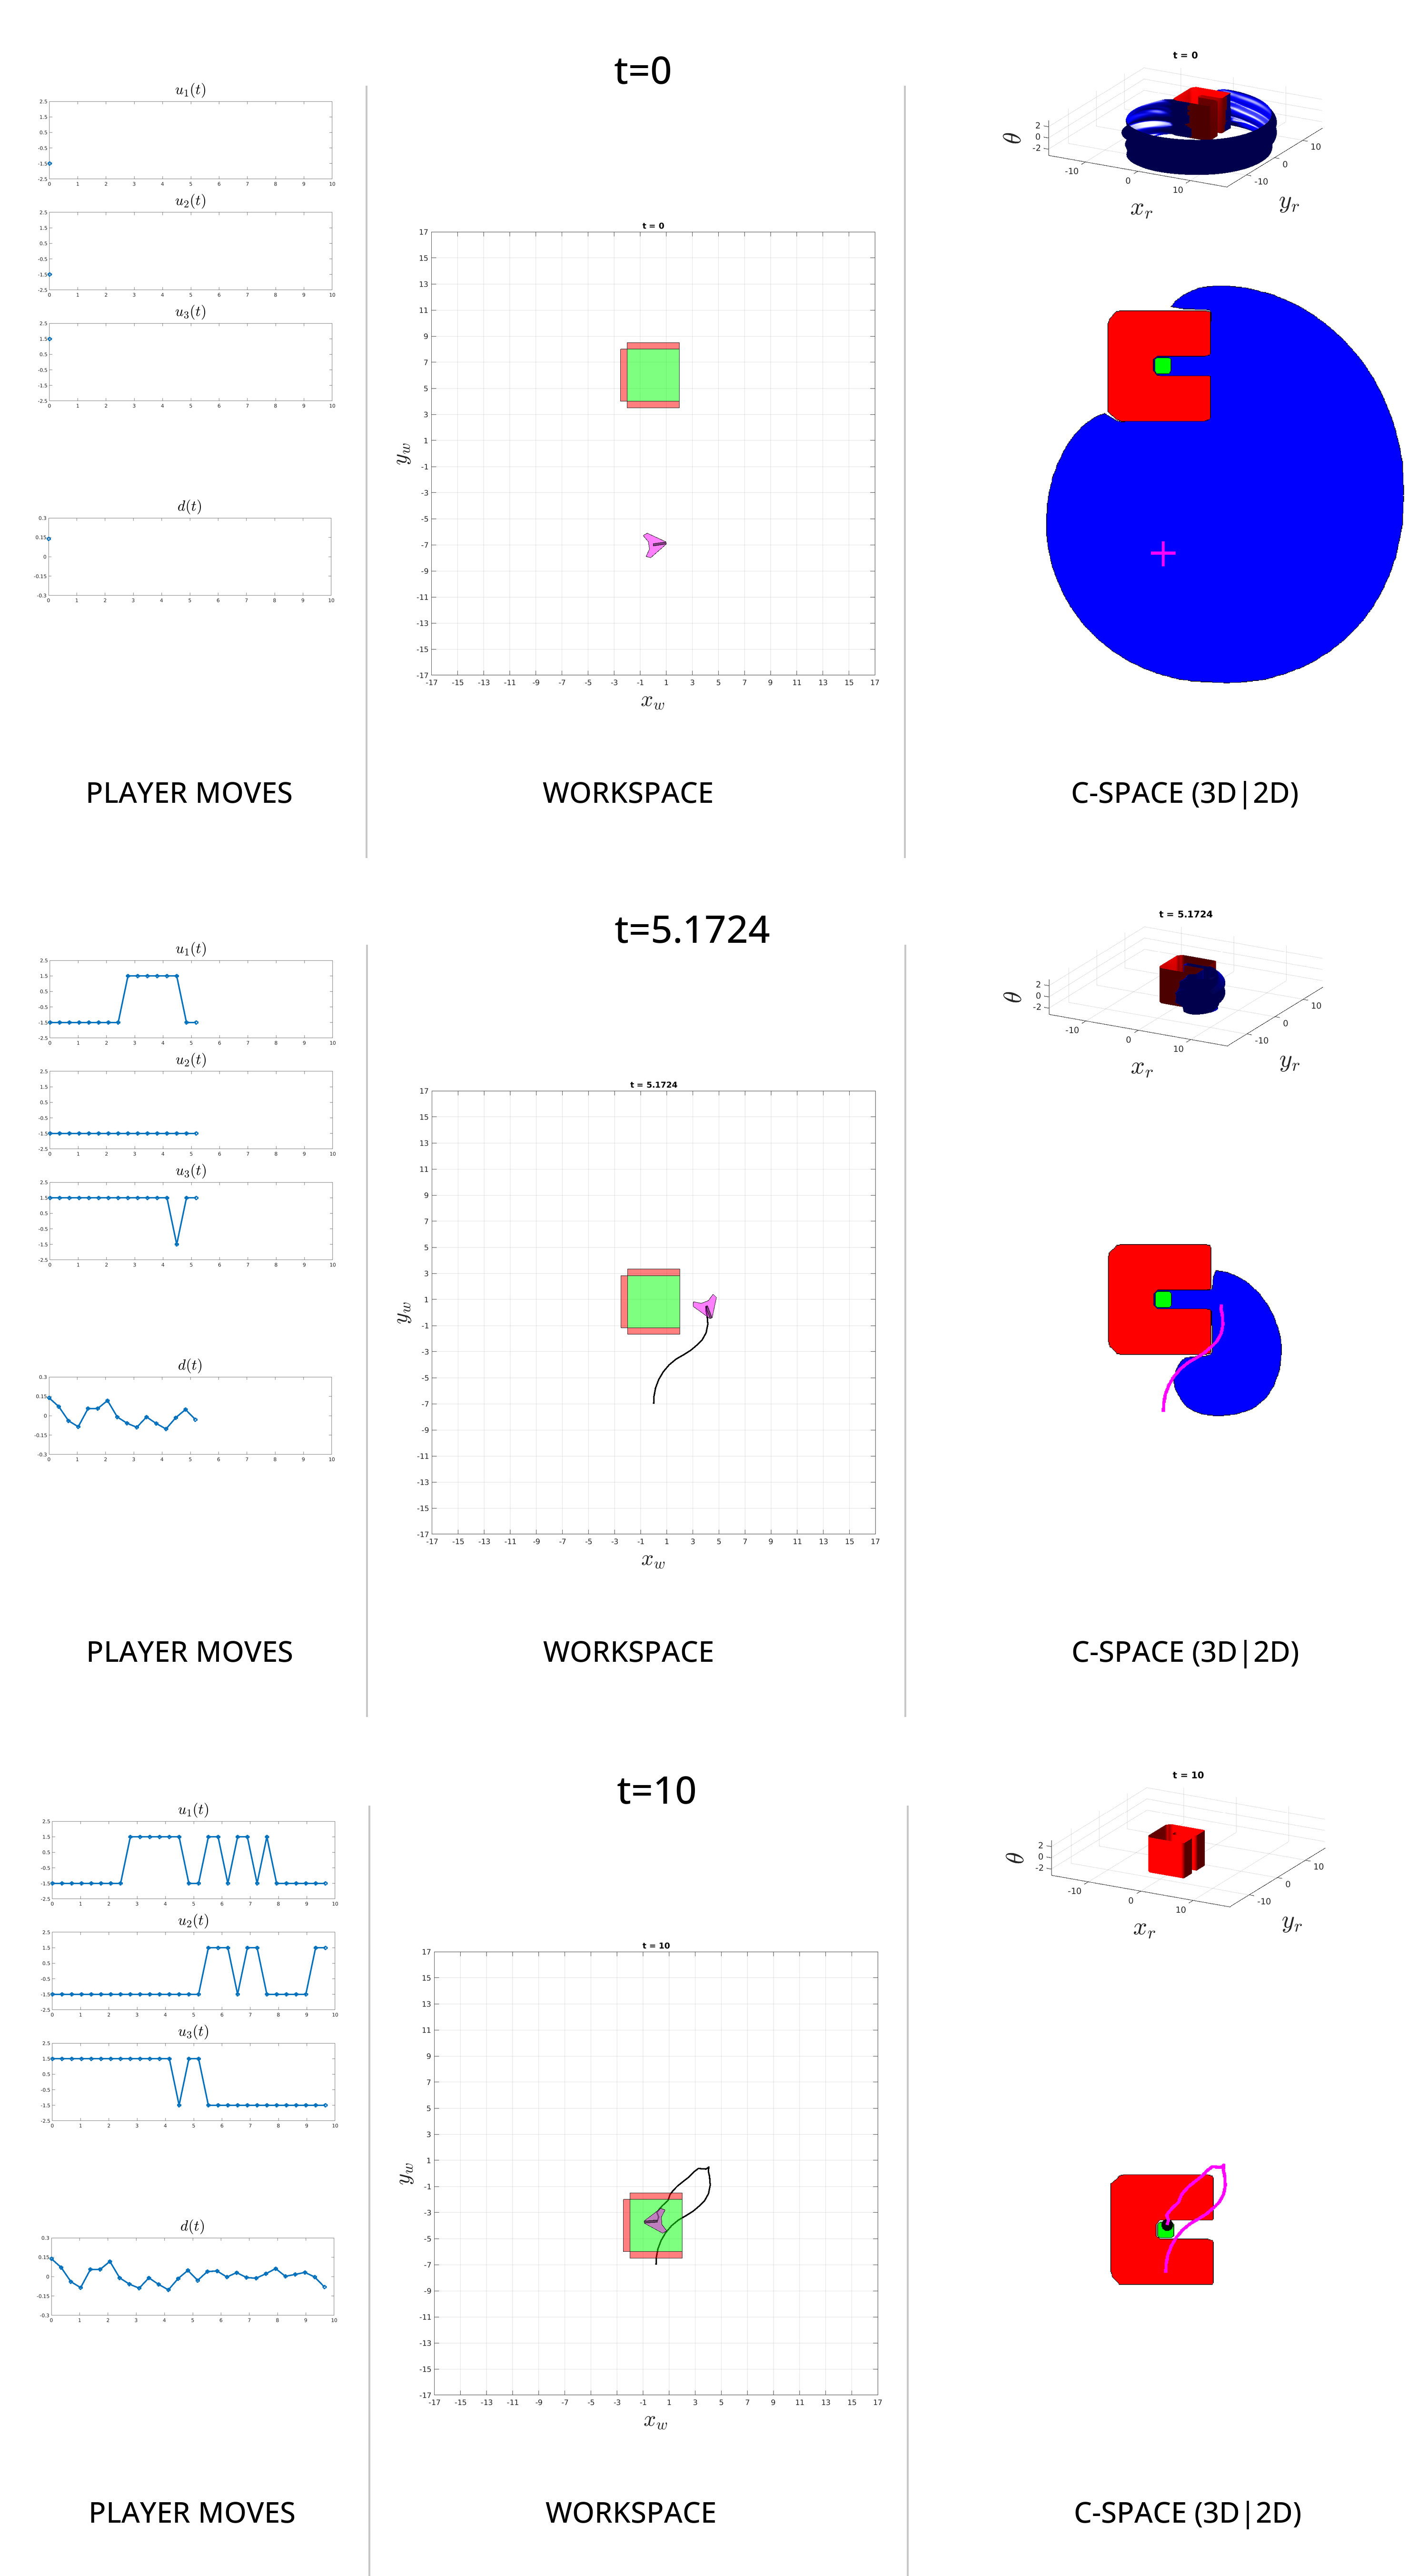
\includegraphics
        [width=0.7\textwidth]
        {figures/dynamic_faraway_ran.png}
    \caption{Dynamic environment, random disturbance. $x_0 = [0, -7, -3]$, $\theta_d \in [-0.1, 0.1]$}
    \label{fig:dynamic_faraway_ran}
\end{figure*}

\begin{figure*}[hp!]
    \centering
    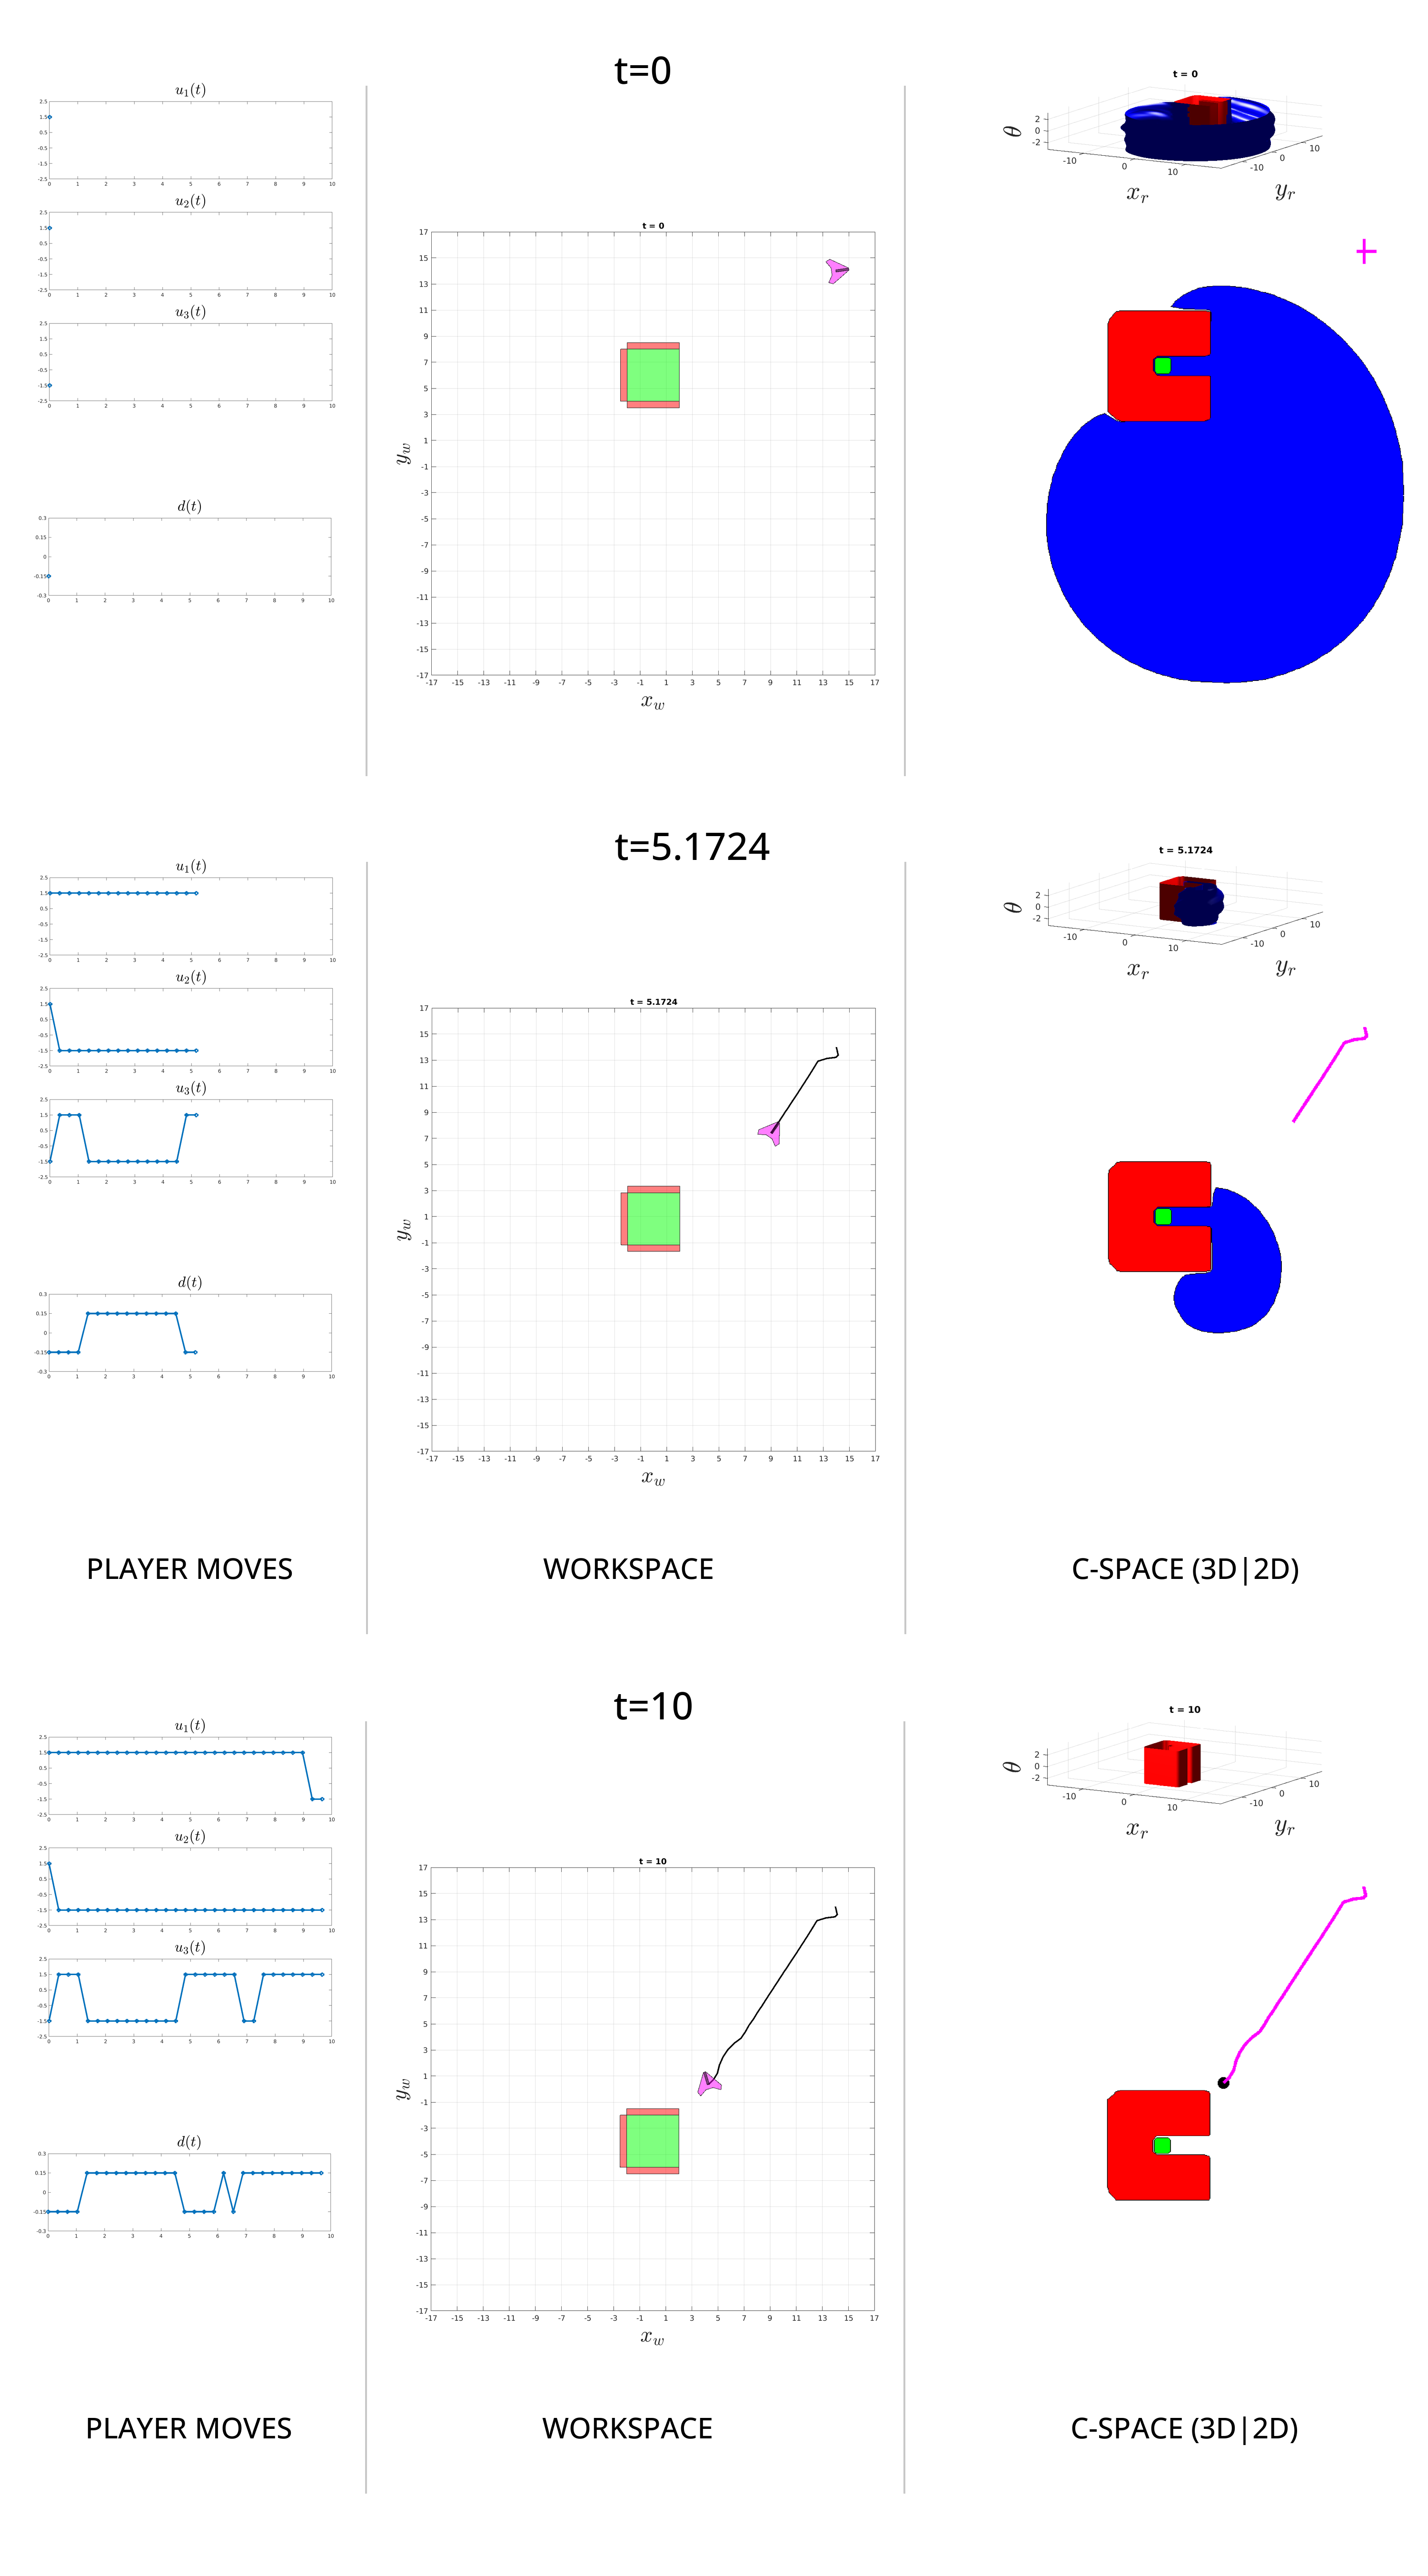
\includegraphics
        [width=0.7\textwidth]
        {figures/dynamic_outside_reach_avoid_set.png}
    \caption{Dynamic environment, optimal disturbance. $x_0 = [14, 14, -3]$, $\theta_d \in [-0.1, 0.1]$ (outside $RAS$)}
    \label{fig:dynamic_outside_reach_avoid_set}
\end{figure*}
